\documentclass[11pt, addpoints]{exam}\usepackage[utf8]{inputenc}
\usepackage[spanish]{babel} % Para idioma español y separación silábica
\usepackage[many]{tcolorbox} % for COLORED BOXES (tikz and xcolor included)
\newtcolorbox{MyBox}{
	fontupper = \bf \color{black}, % font color
    boxrule = 2pt,
    colframe = black,
    rounded corners,
    arc = 12pt
}
\usepackage{qrcode}
\usepackage{amsmath}
\usepackage{graphicx}
\usepackage{amssymb}
\usepackage{geometry}
\geometry{margin=2cm, bottom=3cm}

\begin{document}
	% Macro for conversion of string to barcodes by Code 128 standard
%%%%%%%%%%%%%%%%%%%%%%%%%%%%%%%%%%%%%%%%%%%%%%%%%%%%%%%%%%%%%%%%%
% March 1996                                 (C) Petr Ol\v{s}\'ak

% For user information see the file test128.tex

% Comments at programmer level are included in this file. First you can
% read the end of this file: The description of Code 128 standard.

\wlog{**** Macro for barcodes in "Code 128" by (C) Petr Olsak used ****}

% Declarations:
\newdimen\X            % the module size X,
\newdimen\bcorr        % the bar correction (see bellow).
\newdimen\workdimen \newdimen\barheight   % internal variables
\newtoks\inputtext \newtoks\icode
\newcount\tempnum \newcount\chnum \newcount\chtotal
\newif\ifnext \newif\ifchar
\def\empty{} \def\End{@@end}

% Implicit values:
\X=.33mm         % The X module width.
\bcorr=.020mm    % Bar reduction.
\barheight=1cm % The code height.

% First we declare some tables.
% "\definetable<lab><num> string \relax": Each token from "string" gets a value
% (spaces are ignored). First token gets value <num>, second <num+1>
% and so on. It is possible to reconstruct the value by
% "\csname<lab>\string<token>\endcsname".
\def\definetable#1#2 {\tempnum=#2 \def\temp{#1}\let\next=\repeatdefine \next}
\def\repeatdefine#1{\ifx#1\relax \let\next=\relax \else
  \expandafter\edef\csname\temp\string#1\endcsname{\the\tempnum}%
  \advance\tempnum by1 \fi \next}

%%%%%%%%%%%%%%%%%%%%% Basic tables for Code 128: %%%%%%%%%%%%%%%%%%%%%%%%%%%
\definetable:0  % All input characters from Code B:
  \  ! " \# \$ \% \& ' ( ) * + , - . / 0 1 2 3 4 5 6 7 8 9 : ; < = > ? @
  A B C D E F G H I J K L M N O P Q R S T U V W X Y Z [ \\ ] \^ \_ `
  a b c d e f g h i j k l m n o p q r s t u v w x y z \{ | \} \~ \DEL \relax
\definetable:64 % Other input characters from Code A:
  \NUL \SOH \STX \ETX \EOT \ENQ \ACK \BEL \BS \HT \LF \VT \FF \CR \SO \SI
  \DLE \DCone \DCtwo \DCthree \DCfour \NAK \SYN \ETB \CAN \EM \SUB \ESC
  \FS \GS \RS \US \relax
\definetable:0 \
  \relax    % the \^^M must be the same as \<space>
\definetable:0 \SP \relax  % the \SP is alternative to \<space>
\definetable{D:}0 0123456789 \relax  % Digits
\definetable{B:}0 `abcdefghijklmnopqrstuvwxyz\{\|\}\~ \relax % Only in Code B
\definetable{A:}0  \NUL \SOH \STX \ETX \EOT \ENQ \ACK \BEL \BS \HT \LF \VT
  \FF \CR \SO \SI \DLE \DCone \DCtwo \DCthree \DCfour \NAK \SYN \ETB \CAN
  \EM \SUB \ESC \FS \GS \RS \US \relax % only in code A.
\def\tableofcode#1{\ifcase#1 % The output characters:
  212222\or 222122\or 222221\or 121223\or 121322\or % 0-4
  131222\or 122213\or 122312\or 132212\or 221213\or % 5-9
  221312\or 231212\or 112232\or 122132\or 122231\or % 10-14
  113222\or 123122\or 123221\or 223211\or 221132\or % 15-19
  221231\or 213212\or 223112\or 312131\or 311222\or % 20-24
  321122\or 321221\or 312212\or 322112\or 322211\or % 25-29
  212123\or 212321\or 232121\or 111323\or 131123\or % 30-34
  131321\or 112313\or 132113\or 132311\or 211313\or % 35-39
  231113\or 231311\or 112133\or 112331\or 132131\or % 40-44
  113123\or 113321\or 133121\or 313121\or 211331\or % 45-49
  231131\or 213113\or 213311\or 213131\or 311123\or % 50-54
  311321\or 331121\or 312113\or 312311\or 332111\or % 55-59
  314111\or 221411\or 431111\or 111224\or 111422\or % 60-64
  121124\or 121421\or 141122\or 141221\or 112214\or % 65-69
  112412\or 122114\or 122411\or 142112\or 142211\or % 70-74
  241211\or 221114\or 413111\or 241112\or 134111\or % 75-79
  111242\or 121142\or 121241\or 114212\or 124112\or % 80-84
  124211\or 411212\or 421112\or 421211\or 212141\or % 85-89
  214121\or 412121\or 111143\or 111341\or 131141\or % 90-94
  114113\or 113311\or 411113\or 411311\or 113141\or % 95-99
  114131\or 311141\or 411131\else 00000\fi }        % 100-102
\def\startA{211412}
\def\startB{211214}
\def\startC{211232}
\def\stop{23311120}

% Implementations of tests:
% After "\testchar <lab><token>" the "\ifchar" has following meaning:
% true, if <token> is in digits, only in A or only in B respectively with
% <lab> is {D:}, {A:} or {B:}.
\def\testchar #1#2{\expandafter\ifx\csname#1\string#2\endcsname \relax
          \charfalse \else \chartrue \fi}

% After "\numofdigits string\stop" is used, the \tempnum register contain
% the number of digits from first continuosly group of digits from left in
% "string". If "string" starts with no digit then \tempnum=0.
\def\numofdigits{\tempnum=0 \let\next=\cyklnumber \cyklnumber}
\def\cyklnumber#1{\testchar {D:}#1%
   \ifchar \advance\tempnum by1
   \else \ifx #1\stop\def\next{}%
         \else \def\next##1\stop{}\fi
   \fi \next}

% After "\testnext<lab> string\stop" is used, the "\ifnext" has
% the following meaning:
% 1. <lab> is {A:}: "\ifnext" is true, if first character from "string" is
% only in A code after skip all common characters shared in codeA and B.
% 2. <lab> is {B:}: "\ifnext" is true, if first character from "string" is
% only in B code after skip all common characters shared in codeA and B.
\def\testA{A:}
\def\testnext#1{\nextfalse
  \def\tempA{#1}%
  \ifx\tempA\testA \def\tempB{B:}\else \def\tempB{A:}\fi
  \let\next=\cyklcontrol \next}
\def\cyklcontrol#1{%
   \ifx#1\stop \let\next=\relax
   \else \testchar \tempB #1%
         \ifchar \def\next##1\stop{}%
         \else \testchar \tempA #1%
               \ifchar \nexttrue \def\next##1\stop{}\fi \fi
   \fi \next}

% "\addtok \cs" adds the "\cs," into \icode.
% "\addtoks{string} adds the "string," into \icode. "string" is the number
% of line in table 1, so we re-calculate the current check sum.
% "\addchar <token> adds the numerical value of <token> (declared in
% \definetable:) into \icode. This value is followed by comma too.
\def\addtok#1{\edef\act{\noexpand\icode={\the\icode\noexpand#1,}}\act}
\def\addtoks#1{\edef\act{\noexpand\icode={\the\icode#1,}}\act
  \tempnum=#1 \multiply\tempnum by\chnum
  \advance\chtotal by\tempnum \advance\chnum by 1\relax}
\def\addchar#1{\expandafter\ifx\csname:\string#1\endcsname\relax
  \errmessage{The input token "\string#1" is not included in Code 128
              table, will ignored}%
  \else \expandafter\addtoks\expandafter{\csname:\string#1\endcsname}\fi}

% \code{text} first converts the input text into internal representation in
% \icode. The format of \icode is: "\start,num,num,num,\stop,", where
% "\start" is one of "\startA" or "\startB" or "\startC". The <num>
% represents the line of code table (see standard of Code 128 bellow)
% of output characters. The amount of <num>s is not restricted. The sequence
% is terminated by "\stop,". See to .log for example of this format.
%
% The choice of the start character:
% If next 4 input characters are digits then \startC
% else if the next uncommon char is from code A and not from B then \startA
%      else \startB
% The "next uncommon char" is first character from left which falls
% into code A xor code B
\def\code#1{\inputtext={#1}\wlog{** Code 128 ** input: \the\inputtext}%
  \icode={}\chnum=1
  \numofdigits#1\stop % in \tempnum is the number of digits now
  \ifnum\tempnum>3 \addtok\startC \chtotal=2 \let\Next=\codeC \else
     \testnext{A:} #1\stop
     \ifnext \addtok\startA \chtotal=0 \let\Next=\codeA
     \else \addtok\startB \chtotal=1 \let\Next=\codeB \fi
  \fi \Next #1\End\End}

% There is mode A. Test to change the mode:
% If the next 4 input characters are digits and the number of digits are even
%    then switch to modeC using <codeC>.
% If the next char is from Code B and not from Code A then:
%    if the next uncommnon char is from Code B and not from A then
%         switch to mode B using <codeB>.
%    else include <SHIFT> and stay in mode A.
\def\codeA #1#2#3\End{\addchar#1%
  \numofdigits#2#3\stop
  \ifnum\tempnum>3 \ifodd\tempnum\else
      \addtoks{99}\let\Next=\codeC \fi
  \else \ifx#2\End \let\Next=\finalcode
        \else \testchar{B:} #2%
              \ifchar \testnext{B:} #3\stop
                      \ifnext \addtoks{100}\let\Next=\codeB
                      \else \addtoks{98}\fi \fi \fi \fi
  \Next #2#3\End}

% There is mode B. Test to change the mode:
% If the next 4 input characters are digits and the number of digits are even
%    then switch to modeC using <codeC>
% If the next char is from Code A and not from Code B then:
%    if the next uncommnon char is from Code A and not from B then
%         switch to mode A using <codeA>.
%    else include <SHIFT> and stay in mode B.
\def\codeB #1#2#3\End{\addchar#1%
  \numofdigits#2#3\stop
  \ifnum\tempnum>3 \ifodd\tempnum\else
      \addtoks{99}\let\Next=\codeC \fi
  \else \ifx#2\End \let\Next=\finalcode
        \else \testchar{A:} #2%
              \ifchar \testnext{A:} #3\stop
                      \ifnext \addtoks{101}\let\Next=\codeA
                      \else \addtoks{98}\fi \fi \fi \fi
  \Next #2#3\End}

% There is mode C. Test to change the mode:
% If not next two chars are digits switch to code A or B by following rule:
% If the next uncommon char is from Code A and not from B then
%      switch to mode A using <codeA>
% else switch to mode B using <codeB>
\def\codeC #1#2#3#4\End{\addtoks{#1#2}%
  \ifx#3\End \let\Next=\finalcode
  \else \testchar{D:} #3%
        \ifchar \def\temp{#4}%
                \ifx\temp\empty \switchtoAorB #3\stop
                \else \separate #4\stop
                      \edef\act{\noexpand\testchar{D:}\temp}\act
                      \ifchar
                      \else \switchtoAorB #3#4\stop \fi \fi
        \else \switchtoAorB #3#4\stop \fi
  \fi \Next #3#4\End}
\def\separate#1#2\stop{\def\temp{#1}}
\def\switchtoAorB #1\stop{\testnext{A:} #1\stop
   \ifnext \addtoks{101}\let\Next=\codeA
   \else \addtoks{100}\let\Next=\codeB \fi}

\def\finalcode\End\End{\addchecksum \addtok\stop \wlog{encoded: \the\icode}%
  \expandafter\makecode\the\icode}

% \addchecksum adds the check sum into \icode
\def\addchecksum{\tempnum=\chtotal
  \divide\tempnum by 103 \multiply\tempnum by 103
  \advance\chtotal by-\tempnum \addtoks{\the\chtotal}}

% The \makecode converts the \icode from format "\start,num,num,\stop,"
% into sequence of digits. Each digit repersents the multiple of X module
% size for bar or space if it is at odd or even position. For example
% 21141223311120. It means bar of 2X, space 1X, bar 1X, space 4X and so on.
% This representation of code is stored in macro \internalcode.
\def\makecode#1,{\let\next=\cyklcode \edef\internalcode{#1}\next}
\def\cyklcode#1,{%
  \ifx\stop#1\let\next=\finalmakecode \edef\internalcode{\internalcode\stop}%
  \else \edef\internalcode{\internalcode\tableofcode{#1}}\fi \next}
\def\finalmakecode{\wlog{black-white: \internalcode}%
  \begcode \let\next=\makebars \expandafter\makebars\internalcode}

% \makebars simply makes the \vrules and \kerns of appropriate sizes from
% \internalcode representation. Each width of \vrule is corrected by \bcorr
% and opposite for \kern.
\def\makebars#1#2{\if0#2\let\next=\endcode\fi
  \workdimen=#1\X \advance\workdimen by-\bcorr \vrule width\workdimen
  \workdimen=#2\X \advance\workdimen by \bcorr \kern\workdimen
  \next}

% The begin and end of completed \hbox:
\def\begcode{\hbox\bgroup\vrule height\barheight width0pt}
\def\endcode{\egroup}

% User can use \codetext or \codeothertext instead \code:
\def\codeothertext#1#2{\vbox{\halign{\hfil##\hfil\cr\code{#1}\cr{\tt#2}\cr}}}
\def\codetext#1{\codeothertext{#1}{#1}}

\endinput %%%%%%%%%%%%%%% End of macros %%%%%%%%%%%%%%%%%%%%%%%%%%%%%%%%%%%%

               The description of Code 128 standard
               ************************************

The characters from input string are converted from left to right
to so called "output characters" by table 1 (see below). Each output
character has three bars and spaces. The width of bars and the dimensions
of spaces between bars are significant. This values are expresed by
multiples of basic dimension: so called X module size (see \X in macro).
The multiples varies from 1 to 4. We are using the six digits expression of
output character. It expressed dimensions of bar, space, bar, space, bar,
space. For example 122412 means one output character drawn as: 1X bar, 2X
space, 2X bar, 4X space, 1X bar and 2X space.

The table 1:

num.line  code A    code B    codeC     output character
-------------------------------------------------------
  0       [space]    [space]    00        212222
  1            !         !      01        222122
  2            "         "      02        222221
  3            #         #      03        121223
... and so on ...
 63            _         _      63        111224
 64         \NUL         `      64        111422
 65         \SOH         a      65        121124
 66         \STX         b      66        121421
... and so on ...
 93          \GS         }      93        111341
 94          \RS         ~      94        131141
 95          \US      \DEL      95        114113
 96       <FNC3>    <FNC3>      96        113311
 97       <FNC2>    <FNC2>      97        411113
 98      <SHIFT>   <SHIFT>      98        411311
 99      <codeC>   <codeC>      99        113141
100      <codeB>    <FNC4>   <codeB>      114131
101       <FNC4>   <codeA>   <codeA>      311141
102       <FNC1>    <FNC1>    <FNC1>      411131

The whole table is not presented here because you can simply reconstruct it
from macros.

The columns "code A", "code B", and "code C" inlude all possible input
characters in input string (excluding "special commands" in lines 96--102
written in <angle> braces). The special \TeX{} characters must be escaped
(i.e. user have to write \# and no #). The escaped words (in capitals)
represents so called "control characters" from ASCII. The meaning of this
sequences depends on application. The "special commands" in lines 96--102
written in <angle> braces are not possible in input. They are special for
decoder. The <SHIFT> and <codeA-C> are used in our macro, but <FNC?> are
not because they are reserved for special purposes.

The Code B column is whole expressed in \definetable:0 (see in macro). The
Code A column has the same values in lines 0--63 (capitals, digits and some
other ASCII characters are included here). Code A differ from Code B in
lines 64--102. The lowercase letters and another ASCII characters are
included in "Code B", but control sequences are included in "Code A".
The different part of "Code A" column is expressed in \definetable:64 (see
in macro). The "code C" column includes the digits pairs and corresponds to
number of line in table 1. Two digits in input go to one output character.
The whole "output character" column is expressed in \tableofcode (see in
macro).

The "start character" is appended before each barcode. There are three
types of start character depending on which column of table is used for
next encoding (so called mode). See macros \startA, \startB and \startC.
For examlpe: If \startC is used, next output character represents two
digits in input (codeC mode). If \startB is used, next output character
represents one ASCII character in input (codeB mode). If \startA is used,
next output character represents probably the control sequence in input or
capitals, but not lowercase ASCII (codeA mode).

If some mode for encoding is currently used and next input character is not
included in appropriate column, the "switching command" is included into
sequence of output character. The <SHIFT> command switches from mode A to
B or from B to A only for one next input character and the other input
characters are coded in the same mode (A or B). The <codeA> command
switches to codeA mode definitively unless next switch command is used.
The commands <codeB> and <codeC> makes the same service, but to switch into
mode B or C respectively. All these commands are expessed in table 1.

It is recomended to chose the start character and switching commands by the
way, that the resulting length of code is minimised. There are some
recommendations of this choice. These recommendations are included into our
macros (see the commnets and macros for \code, \codeA, \codeB and \codeC).

The checksum character is added after the end of input string. Finally,
the "stop character" is appended after the end of barcode. This character
has exclusively four bars and not only three. See macro \stop.

The checksum character is calculated from output characters used in the
code. The number of line in table 1 of each output character is asumed. The
start character is covered too, but checksum character itself and the
stop character are not included into calculation. The startA or startB or
startC characters has its number of line 103 or 104 or 105 respectively. Each
output character (more exactly its number of line in table 1) is multiplied
by "weight number" and the total sum is calculated. The weight number of
start character is one. The weight number of first output characet after
start is one too. Second character has weight number two, and so on. The
n-th character has weight number n. The total sum modulo 103 is the line of
the calculated checksum character.

Example for checksum calculation:
Input:    123456
Encoded:  StartC, 12, 34, 56
Total sum of checksum: 105 + 1*12 + 2*34 + 3*56 = 535
Modulo 103: 44
The character from line 44 is apended as checksum.
The whole encoded code: StartC, 12, 34, 56, 44, Stop

%%% End of file.





	\begin{coverpages}
		\begin{center}
			\begin{Large}
				\vspace{-5mm}
				DBS 3rd Exam
			\end{Large}
		\end{center}
		\vspace{5mm}

		\begin{MyBox}
			This exam consists of \numpages{} pages, not including this cover page.  Please go through your copy to make sure that all pages are in good order.  The exam consists of a set of short questions with multiple choices. There are \numpoints{} points, total, on this exam. \\
			Happy solving!
		\end{MyBox}

		\vspace{10mm}
		\noindent
		Name:\enspace\hrulefill \\
		\\
		Date:\enspace\hrulefill
		\vspace{5mm}
		\begin{center}
			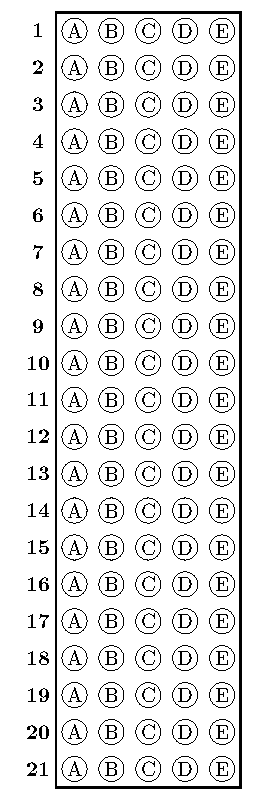
\includegraphics{../answer_table}

			\vspace{3mm}
			\leavevmode \hspace{5mm} \codetext{33CE8F}
		\end{center}
	\end{coverpages}

	\footer{} {Page \thepage\ of \numpages} {\iflastpage{3rd exam.}{Please go on to the next page\ldots}}

	\centering
	\textbf{\Large Pontificia Universidad Javeriana}\\
	\textbf{\Large Databases} \\
	\textbf{\large 2025 -- 10} \\
	\textbf{\large 3rd Exam} \\
	\textbf{Code: 33CE8F}


	\begin{questions}
		\question[1] ¿Cuál es la función principal de un trigger de validación?
\begin{choices}
\choice Actualizar múltiples tablas
\CorrectChoice Rechazar datos inválidos antes de insertarlos
\choice Crear índices automáticamente
\choice Ejecutar vistas materializadas
\end{choices}
		\question[1] ¿Cuál es el objetivo de la propiedad de aislamiento en una transacción?
\begin{choices}
\CorrectChoice Asegurar que las transacciones se ejecuten sin interferencias
\choice Eliminar bloqueos de registros
\choice Reducir el tamaño de la base de datos
\choice Aumentar la velocidad de lectura
\end{choices}
		\question[1] ¿Cuál de las siguientes operaciones de MongoDB elimina un solo documento?
\begin{choices}
\choice \texttt{removeOne}
\CorrectChoice \texttt{deleteOne}
\choice \texttt{deleteAll}
\choice \texttt{dropOne}
\end{choices}
		\question[1] ¿Qué tipo de trigger se utiliza comúnmente para reemplazar una operación en una vista?
\begin{choices}
\choice AFTER
\CorrectChoice INSTEAD OF
\choice BEFORE
\choice REPLACE
\end{choices}
		\question[1] ¿Qué tipo de serializabilidad se basa en el orden de las operaciones?
\begin{choices}
\CorrectChoice Serializabilidad por Conflicto
\choice Serializabilidad por Vista
\choice Serializabilidad Predictiva
\choice Serialización Total
\end{choices}
		\question[1] ¿Qué ocurre si un trigger lanza una excepción?
\begin{choices}
\choice Se ignora el error y continúa
\CorrectChoice La transacción se revierte
\choice El trigger se desactiva automáticamente
\choice El error solo se registra en el log
\end{choices}
		\question[1] ¿Cuál de los siguientes NO es un tipo de trigger en PostgreSQL?
\begin{choices}
\choice BEFORE
\choice AFTER
\choice INSTEAD OF
\CorrectChoice UNTIL
\end{choices}
		\question[1] ¿Qué tipo de base de datos NoSQL es mejor para representar relaciones entre entidades?
\begin{choices}
\choice Columna
\CorrectChoice Grafo
\choice Clave-valor
\choice Documental
\end{choices}
		\question[1] ¿Cuál de las siguientes afirmaciones describe mejor las bases de datos NoSQL?
\begin{choices}
\choice Son exclusivamente relacionales
\CorrectChoice Están diseñadas para datos no estructurados y escalabilidad horizontal
\choice Solo funcionan con tablas normalizadas
\choice Requieren JOINs para todas las consultas
\end{choices}
		\question[1] ¿Cuál de los siguientes escenarios es mejor para una base de datos grafo?
\begin{choices}
\choice Gestión de inventarios
\choice Análisis contable
\CorrectChoice Recomendación de amigos en redes sociales
\choice Registro de sensores
\end{choices}
		\question[1] ¿Qué tipo de base de datos NoSQL utiliza documentos tipo JSON/BSON?
\begin{choices}
\choice Redis
\CorrectChoice MongoDB
\choice Neo4j
\choice Cassandra
\end{choices}
		\question[1] ¿Qué nivel de aislamiento permite lecturas sucias?
\begin{choices}
\CorrectChoice Read Uncommitted
\choice Serializable
\choice Repeatable Read
\choice Read Committed
\end{choices}
		\question[1] ¿Qué significa la propiedad de durabilidad?
\begin{choices}
\choice La transacción se puede revertir fácilmente.
\choice La base de datos se reinicia después de cada transacción.
\CorrectChoice Los cambios persisten incluso ante fallos del sistema.
\choice Las transacciones se ejecutan en paralelo.
\end{choices}
		\question[1] ¿Qué lenguaje se utiliza para definir funciones de trigger en PostgreSQL?
\begin{choices}
\CorrectChoice PL/pgSQL
\choice T-SQL
\choice PL/SQL
\choice SQLServer
\end{choices}
		\question[1] ¿Qué tipo de datos es ideal para una base de datos documental?
\begin{choices}
\CorrectChoice Estructura jerárquica y flexible
\choice Datos puramente relacionales
\choice Transacciones bancarias
\choice Lecturas secuenciales masivas
\end{choices}
		\question[1] ¿Qué método de MongoDB retorna todos los documentos de una colección?
\begin{choices}
\choice \texttt{listAll()}
\CorrectChoice \texttt{find()}
\choice \texttt{getAll()}
\choice \texttt{queryAll()}
\end{choices}
		\question[1] ¿Qué tipo de consistencia proporciona mayor rendimiento pero menor precisión?
\begin{choices}
\CorrectChoice Read Uncommitted
\choice Serializable
\choice Repeatable Read
\choice Strict Serializability
\end{choices}
		\question[1] ¿Cuál es una de las propiedades ACID?
\begin{choices}
\choice Adaptabilidad
\CorrectChoice Atomicidad
\choice Agilidad
\choice Asincronía
\end{choices}
		\question[1] ¿Qué nivel de aislamiento previene todos los problemas de lectura?
\begin{choices}
\CorrectChoice Serializable
\choice Repeatable Read
\choice Read Committed
\choice Read Uncommitted
\end{choices}
		\question[1] ¿Cuál de los siguientes usos NO es recomendado para triggers?
\begin{choices}
\choice Validar datos
\CorrectChoice Ejecutar lógica de negocio compleja
\choice Auditar cambios
\choice Prevenir eliminaciones
\end{choices}
	\end{questions}

	\vspace{5mm}
	\noindent \textbf{End of Exam}

\end{document}
